\documentclass[12pt,a4paper]{report}
\usepackage{amssymb}
\usepackage{amsthm}
\usepackage{amsmath}
\usepackage{enumitem}
\usepackage{graphicx}
\usepackage{tikz}
\usetikzlibrary{plotmarks}
\usetikzlibrary{patterns,shapes.arrows}
\usepackage{pgfplots}


\DeclareMathOperator{\spn}{span}


\begin{document}
\noindent Johannes Kasimir
	

	
\section*{P1: Relation between "Jacobi DN" and "Gau\ss-Seidel DN" iterates }

For the regular (GS-) DN iteration on two domains $\Omega_1$ and $\Omega_2$, the iteration is described by the following three equations
\begin{align}
\label{gs1}
\mathbf{A}_{II}^{(1)} \mathbf{u}_I^{(1),k+1} = \mathbf{f}^{(1)}_I - \mathbf{A}_{I\Gamma}^{(1)}\mathbf{u}^k_\Gamma \\
\label{gs2}
\mathbf{A}_{II}^{(2)} \mathbf{u}_I^{(2),k+1} = \mathbf{f}^{(2)}_I - \mathbf{A}_{I\Gamma}^{(2)}\mathbf{u}^{k+1}_\Gamma \\
\label{gs3}
\mathbf{A}_{\Gamma I}^{(2)} \mathbf{u}_I^{(2),k+1} + \mathbf{A}_{\Gamma \Gamma}^{(2)} \mathbf{u}_\Gamma^{k+1}= \mathbf{f}_\Gamma - \mathbf{A}_{\Gamma I}^{(1)}\mathbf{u}^{(1),k+1}_I - \mathbf{A}_{\Gamma \Gamma}^{(1)} \mathbf{u}_\Gamma^{k}.
\end{align}
The sense in which this is GS is that \eqref{gs3} depends on the solution $\mathbf{u}_I^{(1),k+1}$ and $\mathbf{u}_\Gamma^{k}$ to the Dirichlet problem at the same step in the iteration. To make this "Jacobi" we replace $\mathbf{u}_I^{(1),k+1}$ and $\mathbf{u}_\Gamma^{k}$ with the solution $\mathbf{u}_I^{(1),k}$ and $\mathbf{u}_\Gamma^{k-1}$ to the Dirichlet problem from the previous step $k$. Doing this we obtain the system defining the Jacobi-DN iteration below
\begin{align}
\label{j1}
\mathbf{A}_{II}^{(1)} \mathbf{u}_I^{(1),k+1} = \mathbf{f}^{(1)}_I - \mathbf{A}_{I\Gamma}^{(1)}\mathbf{u}^k_\Gamma \\
\label{j2}
\mathbf{A}_{II}^{(2)} \mathbf{u}_I^{(2),k+1} = \mathbf{f}^{(2)}_I - \mathbf{A}_{I\Gamma}^{(2)}\mathbf{u}^{k+1}_\Gamma \\
\label{j3}
\mathbf{A}_{\Gamma I}^{(2)} \mathbf{u}_I^{(2),k+1} + \mathbf{A}_{\Gamma \Gamma}^{(2)} \mathbf{u}_\Gamma^{k+1}= \mathbf{f}_\Gamma - \mathbf{A}_{\Gamma I}^{(1)}\mathbf{u}^{(1),k}_I - \mathbf{A}_{\Gamma \Gamma}^{(1)} \mathbf{u}_\Gamma^{k-1}.
\end{align}

The above two equation systems each define a linear iteration on $\mathbf{u}_\Gamma^{k}$. The GS-DN system \eqref{gs1}-\eqref{gs3} gives the iteration
\begin{align}
\label{itgs}
(\mathbf{A}_{\Gamma \Gamma}^{(2)} - \mathbf{A}_{\Gamma I}^{(2)} \mathbf{A}_{II}^{(2)-1} \mathbf{A}_{I\Gamma}^{(2)}) \mathbf{u}_\Gamma^{k+1} = \\
\nonumber
 (\mathbf{A}_{\Gamma I}^{(1)}\mathbf{A}_{II}^{(1)-1}\mathbf{A}_{I\Gamma}^{(1)} - \mathbf{A}_{\Gamma \Gamma}^{(1)}) \mathbf{u}_\Gamma^{k} + \mathbf{f}_\Gamma - \mathbf{A}_{\Gamma I}^{(1)}\mathbf{A}_{II}^{(1)-1} \mathbf{f}^{(1)}_I  - \mathbf{A}_{\Gamma I}^{(2)} \mathbf{A}_{II}^{(2)-1}\mathbf{f}^{(2)}_I
\end{align}
and the Jacobi-DN system \eqref{j1}-\eqref{j3} gives the iteration
\begin{align}
(\mathbf{A}_{\Gamma \Gamma}^{(2)} - \mathbf{A}_{\Gamma I}^{(2)} \mathbf{A}_{II}^{(2)-1} \mathbf{A}_{I\Gamma}^{(2)}) \mathbf{u}_\Gamma^{k+1} = \\
\nonumber
(\mathbf{A}_{\Gamma I}^{(1)}\mathbf{A}_{II}^{(1)-1}\mathbf{A}_{I\Gamma}^{(1)} - \mathbf{A}_{\Gamma \Gamma}^{(1)}) \mathbf{u}_\Gamma^{k-1} + \mathbf{f}_\Gamma - \mathbf{A}_{\Gamma I}^{(1)}\mathbf{A}_{II}^{(1)-1} \mathbf{f}^{(1)}_I  - \mathbf{A}_{\Gamma I}^{(2)} \mathbf{A}_{II}^{(2)-1}\mathbf{f}^{(2)}_I.
\end{align}
This shows that if GS-DN and Jacobi-DN are applied to the same problem and provided the same $\mathbf{u}_{\Gamma}^0$ then $\mathbf{u}_{\Gamma(Jacobi)}^2 = \mathbf{u}_{\Gamma(Gau\ss-Seidel)}^1$ and so on for all $k$. If the iteration converges then GS-DN converges twice as fast as J-DN.

\section*{P2: Matrix splitting defining DN iteration }

Equations \eqref{gs1}-\eqref{gs3} above gives that
\begin{equation}
\mathbf{B} =
\begin{bmatrix}
\mathbf{A}_{II}^{(1)} & \mathbf{0} & \mathbf{0} \\
\mathbf{0} & \mathbf{A}_{II}^{(2)} & \mathbf{A}_{I\Gamma}^{(2)} \\
\mathbf{A}_{\Gamma I}^{(1)} & \mathbf{A}_{\Gamma I}^{(2)} & \mathbf{A}_{\Gamma \Gamma}^{(2)}´
\end{bmatrix}.
\end{equation}
This again illustrates what is "Gau\ss-Seidel" about the method. But also shows that it is not \textit{the} Gau\ss-Seidel matrix splitting method.

\section*{P3}

Niklas Kotarsky and I worked together on this task.\\

We calculated the stationary heat distribution in the 3 rooms using the finite element solver for the Poisson equation from last week with a few tweaks:
\begin{itemize}
	\item support for rectangular domains,
	\item option to apply boundary conditions in the form of a raw vectors instead of node values,
	\item ability to extract heat flux in node points (in other words, the vector $\mathbf{A}^{(1)}_{\Gamma I}\mathbf{u}_I + \mathbf{A}^{(1)}_{\Gamma\Gamma}\mathbf{u}_\Gamma$ required for the DN iteration),
	\item variable heat conductivity $\lambda$.
\end{itemize}

    Since the finite element method was described last week, and the discrete DN iteration is described in problem 1, we will focus on the issues encountered when solving the 3 room problem.
    
    \subsection*{How to interpret the boundary values?}
    The prescribed boundary value is discontinuous between the wall and the window and the walls and the radiators. This makes the condition impossible to enforce on all boundaries simultaneously since our discretization can only represent continuous functions. We chose to enforce the wall boundary conditions wherever ambiguity arose. This means the corners all have wall boundary conditions. As can be seen in figure \ref{WindowWall} the unknown on the bottom shared by $\Omega_1$ and $\Omega_2$ was also assigned the wall boundary condition.
    
    \subsection*{Do we have convergence?}
    We measured error as $e_k = ||\mathbf{u}_\Gamma^{k} - \mathbf{u}_\Gamma^{last}||_{l_2}$. We can see that after a number of iterations this values reaches the computer epsilon, see figure \ref{fig:convergence}. This shows we have reached the fixed point of the iteration in equation \eqref{itgs} which shows we have found the solution to the monolithic problem.\\
 
	\subsection*{Results}
	Figure \ref{tempdist} shows the solution to the problem given in task 3. If heat conductivity is 1 in all rooms the optimal relaxation parameter is 0.47 \ref{fig:vary_theta}. Changing the heat conductivity in room 2 to $0.0243$ changes the optimal relaxation parameter to 0.02, which can be seen in figure \ref{fig:vary_theta_other_heat_cond}.  
	
	
	\begin{figure}
		\centering
		% This file was created with tikzplotlib v0.9.15.
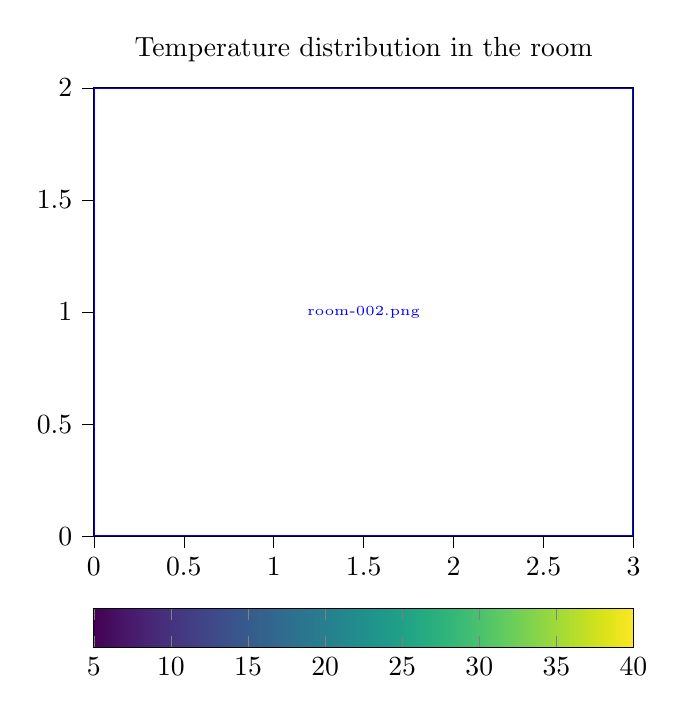
\begin{tikzpicture}

\begin{axis}[
colorbar horizontal,
colormap/viridis,
point meta max=40.0000000000002,
point meta min=4.99999999999999,
tick align=outside,
tick pos=left,
title={Temperature distribution in the room},
x grid style={white!69.0196078431373!black},
xmin=0, xmax=3,
xtick style={color=black},
y grid style={white!69.0196078431373!black},
ymin=0, ymax=2,
ytick style={color=black}
]
\addplot graphics [includegraphics cmd=\pgfimage,xmin=0, xmax=3, ymin=0, ymax=2] {room-002.png};
\end{axis}

\end{tikzpicture}

		\caption{The temperature of the 3 different rooms.}
		\label{tempdist}
	\end{figure}
	
	\begin{figure}
		\centering
		% This file was created with tikzplotlib v0.9.15.
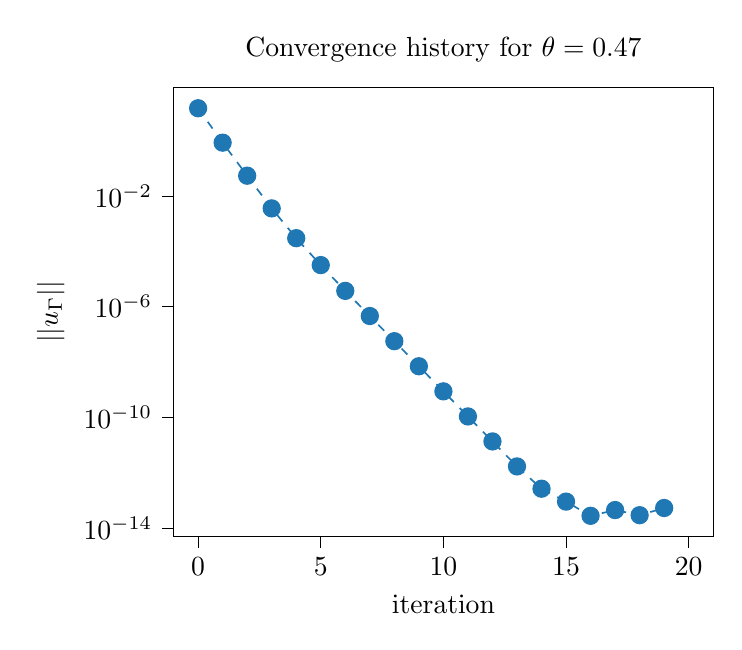
\begin{tikzpicture}

\definecolor{color0}{rgb}{0.12156862745098,0.466666666666667,0.705882352941177}

\begin{axis}[
log basis y={10},
tick align=outside,
tick pos=left,
title={Convergence history for \(\displaystyle \theta=0.47\)},
x grid style={white!69.0196078431373!black},
xlabel={iteration},
xmin=-1, xmax=21,
xtick style={color=black},
y grid style={white!69.0196078431373!black},
ylabel={\(\displaystyle ||u_\Gamma||\)},
ymin=5.05106520789818e-15, ymax=79.606009556297,
ymode=log,
ytick style={color=black}
]
\addplot [semithick, color0, dashed, mark=*, mark size=3, mark options={solid}]
table {%
0 14.611439704895
1 0.833687126636505
2 0.0534031912684441
3 0.00352828809991479
4 0.000295949837891385
5 3.15005527227186e-05
6 3.68922428606311e-06
7 4.55424867595866e-07
8 5.61464652548693e-08
9 6.97394009208097e-09
10 8.64427307512017e-10
11 1.07227185464076e-10
12 1.34170469873185e-11
13 1.67806469674597e-12
14 2.62396305855325e-13
15 8.97543215964969e-14
16 2.75192263182907e-14
17 4.44444590993413e-14
18 2.90259014198123e-14
19 5.2695220691297e-14
};
\end{axis}

\end{tikzpicture}

		\caption{\label{fig:convergence}Example convergence history of the iteration. The error is calculated compared to $u_\Gamma^k$ in the last iteration.}
	\end{figure}
	
	\begin{figure}
		\centering
		% This file was created with tikzplotlib v0.9.15.
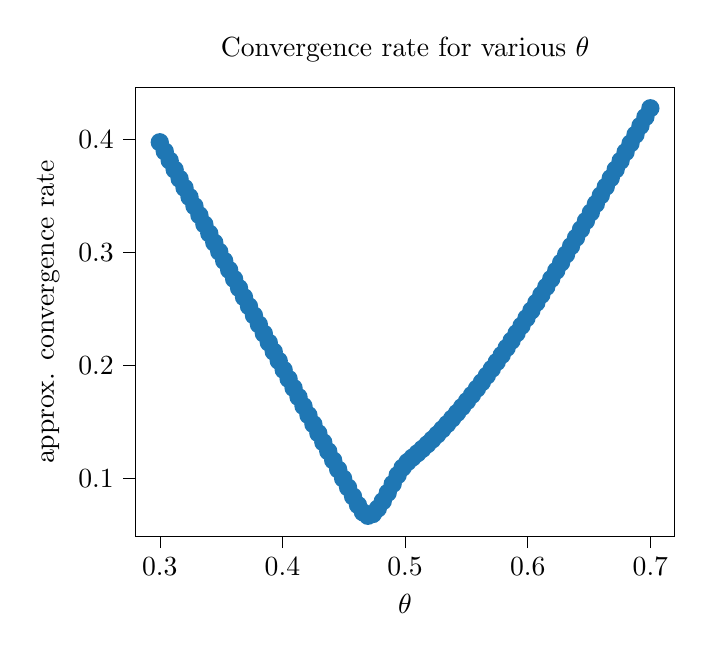
\begin{tikzpicture}

\definecolor{color0}{rgb}{0.12156862745098,0.466666666666667,0.705882352941177}

\begin{axis}[
tick align=outside,
tick pos=left,
title={Convergence rate for various \(\displaystyle \theta\)},
x grid style={white!69.0196078431373!black},
xlabel={\(\displaystyle \theta\)},
xmin=0.28, xmax=0.72,
xtick style={color=black},
y grid style={white!69.0196078431373!black},
ylabel={approx. convergence rate},
ymin=0.0486727472381146, ymax=0.44559116074117,
ytick style={color=black}
]
\addplot [semithick, color0, mark=*, mark size=3, mark options={solid}, only marks]
table {%
0.299999952316284 0.397450804710388
0.304040431976318 0.389367580413818
0.308080792427063 0.381285786628723
0.312121152877808 0.373205542564392
0.316161632537842 0.365127086639404
0.320201992988586 0.357050180435181
0.324242353439331 0.3489750623703
0.328282833099365 0.340901732444763
0.33232319355011 0.332830190658569
0.336363673210144 0.324760675430298
0.340404033660889 0.316693067550659
0.344444513320923 0.308627367019653
0.348484873771667 0.300563931465149
0.352525234222412 0.292502522468567
0.356565713882446 0.284443378448486
0.360606074333191 0.276386499404907
0.364646434783936 0.268332004547119
0.36868691444397 0.260279893875122
0.372727274894714 0.252230167388916
0.376767635345459 0.24418306350708
0.380808115005493 0.236138582229614
0.384848475456238 0.228096842765808
0.388888835906982 0.220057845115662
0.392929315567017 0.212021589279175
0.396969676017761 0.203988313674927
0.401010036468506 0.195957779884338
0.40505051612854 0.187930345535278
0.409090876579285 0.179905652999878
0.413131356239319 0.171884059906006
0.417171716690063 0.163865208625793
0.421212077140808 0.155849099159241
0.425252556800842 0.147835493087769
0.429292917251587 0.139823913574219
0.433333396911621 0.131814241409302
0.437373757362366 0.123805522918701
0.44141411781311 0.115797162055969
0.445454597473145 0.107788801193237
0.449494957923889 0.0997823476791382
0.453535318374634 0.0917906761169434
0.457575798034668 0.0838704109191895
0.461616158485413 0.0762566328048706
0.465656518936157 0.0698270797729492
0.469696998596191 0.0667145252227783
0.473737359046936 0.0682775974273682
0.477777719497681 0.0731250047683716
0.481818199157715 0.0796537399291992
0.485858559608459 0.0870462656021118
0.489898920059204 0.0949231386184692
0.493939399719238 0.10271167755127
0.497979760169983 0.109336256980896
0.502020120620728 0.114286303520203
0.506060600280762 0.118287682533264
0.510101079940796 0.122083187103271
0.514141440391541 0.125972867012024
0.518181800842285 0.130033373832703
0.522222280502319 0.134271621704102
0.526262640953064 0.138678550720215
0.530303001403809 0.143244385719299
0.534343481063843 0.147962093353271
0.538383841514587 0.152826905250549
0.542424201965332 0.157836198806763
0.546464681625366 0.162988066673279
0.550505042076111 0.168280959129333
0.554545402526855 0.173712968826294
0.55858588218689 0.179281830787659
0.562626242637634 0.184984683990479
0.566666603088379 0.190818548202515
0.570707082748413 0.196779489517212
0.574747562408447 0.202863335609436
0.578787803649902 0.209065437316895
0.582828283309937 0.215381264686584
0.586868762969971 0.221805453300476
0.590909004211426 0.228332996368408
0.59494948387146 0.234958529472351
0.598989963531494 0.241676926612854
0.603030323982239 0.248482704162598
0.607070684432983 0.25537097454071
0.611111164093018 0.262336492538452
0.615151524543762 0.269374489784241
0.619191884994507 0.276480197906494
0.623232364654541 0.283649325370789
0.627272725105286 0.2908775806427
0.63131308555603 0.298160910606384
0.635353565216064 0.305495500564575
0.639393925666809 0.312878012657166
0.643434286117554 0.320304870605469
0.647474765777588 0.327773213386536
0.651515126228333 0.335279941558838
0.655555486679077 0.342822551727295
0.659595966339111 0.350398540496826
0.663636445999146 0.358005404472351
0.667676687240601 0.365641117095947
0.671717166900635 0.373303651809692
0.675757646560669 0.380991220474243
0.679798007011414 0.388701915740967
0.683838367462158 0.396434187889099
0.687878847122192 0.404186487197876
0.691919207572937 0.411957383155823
0.695959568023682 0.419745445251465
0.700000047683716 0.427549362182617
};
\end{axis}

\end{tikzpicture}

		\caption{The DN iterations convergence rate's dependency of the relaxation parameter $\theta$.}
		\label{fig:vary_theta}
	\end{figure}
	
	
	\begin{figure}
		\centering
		% This file was created with tikzplotlib v0.9.15.
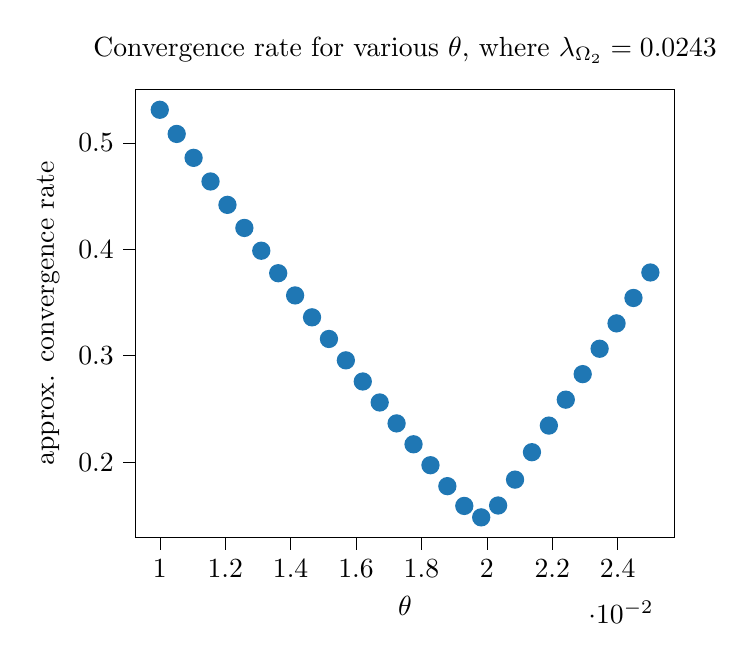
\begin{tikzpicture}

\definecolor{color0}{rgb}{0.12156862745098,0.466666666666667,0.705882352941177}

\begin{axis}[
tick align=outside,
tick pos=left,
title={Convergence rate for various \(\displaystyle \theta\), where \(\displaystyle \lambda_{\Omega_2} = 0.0243\)},
x grid style={white!69.0196078431373!black},
xlabel={\(\displaystyle \theta\)},
xmin=0.00925, xmax=0.02575,
xtick style={color=black},
y grid style={white!69.0196078431373!black},
ylabel={approx. convergence rate},
ymin=0.129080228806446, ymax=0.550183415135969,
ytick style={color=black}
]
\addplot [semithick, color0, mark=*, mark size=3, mark options={solid}, only marks]
table {%
0.00999999046325684 0.531042337417603
0.0105172395706177 0.508358120918274
0.0110344886779785 0.48590612411499
0.0115517377853394 0.463699698448181
0.0120689868927002 0.441750526428223
0.012586236000061 0.420068502426147
0.0131034851074219 0.398660778999329
0.0136207342147827 0.3775315284729
0.0141379833221436 0.356680870056152
0.0146551132202148 0.336103320121765
0.0151723623275757 0.315786480903625
0.0156896114349365 0.295708894729614
0.0162068605422974 0.27583646774292
0.0167241096496582 0.256119847297668
0.017241358757019 0.236492156982422
0.0177586078643799 0.216872811317444
0.0182758569717407 0.197197079658508
0.0187931060791016 0.177547812461853
0.0193103551864624 0.1589674949646
0.0198276042938232 0.148221254348755
0.0203448534011841 0.159374117851257
0.0208621025085449 0.183669090270996
0.0213793516159058 0.20942211151123
0.0218966007232666 0.234427332878113
0.0224138498306274 0.2587730884552
0.0229309797286987 0.282762050628662
0.0234482288360596 0.306605458259583
0.0239654779434204 0.33042573928833
0.0244827270507812 0.35429048538208
0.0249999761581421 0.378235459327698
};
\end{axis}

\end{tikzpicture}

		\caption{Changing the problem parameters changes the optimal $\theta$.}
		\label{fig:vary_theta_other_heat_cond}
	\end{figure}
	
	\begin{figure}
		\centering
		% This file was created with tikzplotlib v0.9.15.
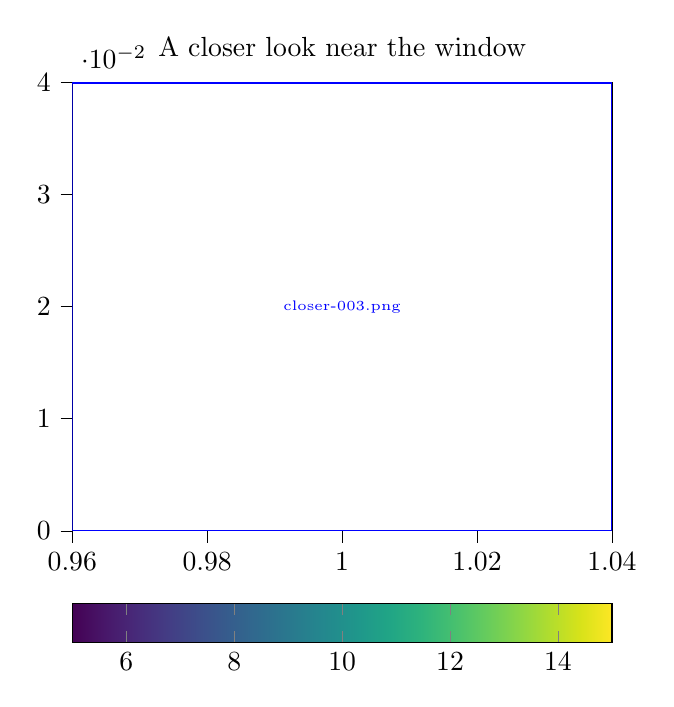
\begin{tikzpicture}

\begin{axis}[
colorbar horizontal,
colormap/viridis,
point meta max=15.0000000000001,
point meta min=5,
tick align=outside,
tick pos=left,
title={A closer look near the window},
x grid style={white!69.0196078431373!black},
xmin=0.96, xmax=1.04,
xtick style={color=black},
y grid style={white!69.0196078431373!black},
ymin=0, ymax=0.04,
ytick style={color=black}
]
\addplot graphics [includegraphics cmd=\pgfimage,xmin=0.96, xmax=1.04, ymin=0, ymax=0.04] {closer-003.png};
\end{axis}

\end{tikzpicture}

		\caption{We chose to count the point (1, 0) as part of the wall with a boundary condition of $15^\circ C$ on both $\Omega_1$ and $\Omega_2$.}
		\label{WindowWall}
	\end{figure}
	

	
\end{document}